\section{Nos tests}

Nous avons mis en place divers outils pour contrôler notre implémentation :
\begin{itemize}
    \item Chaque \emph{commit} sera vérifier par des pipelines de \emph{GitLab}. Cet outil compile le code proposé sur une machine afin de voir si le code suggérer n'a aucune erreur de compilation.
    \item L'implémentation de notre \emph{backend} est contrôlé par le framework \emph{NYC}. Nos tests sont surveillés par le framework et nous donne le résultat de \emph{coverage} pour chaque fichier testé.
\end{itemize}

\subsection{Test unitaire}

Consigne : description des tests, discussion de leurs résultats, explication des problèmes, des défauts et bugs. Pour chacun des tests avec : (1) spécification et buts du test ;
(2) cas de tests (données) utilisé ; (3) scénario du test ; (4) analyse du test et les moyens de mise en œuvre de cette analyse.

\subsubsection{Vérification des fichiers dans le fichier \emph{src}}

\begin{center}
    \centering
    \begin{tabular}[h]{|m{4cm}|m{12cm}|} 
        \hline
        \rowcolor[HTML]{F8B400}
        \textbf{But} & Vérifier si les fichiers possède le bon format (\texttt{.ts}) dans le dossier \texttt{src/main} \\
        \hline
        \hline
        \rowcolor[HTML]{F7F7F7}
        Entrée & Un ensemble de fichiers \\
        \hline
        \rowcolor[HTML]{F7F7F7}
        Scénario & En cas de mauvais format dans le dossier, on affiche les fichiers qui ne respectent pas le format \texttt{.ts}\\
        \hline
        \rowcolor[HTML]{F7F7F7}
        Analyse du test & Parcours d'un dossier en ajoutant dans une liste les fichiers qui ne respecte pas la condition \\
        \hline
    \end{tabular}
\end{center}

\begin{center}
    \centering
    \begin{tabular}[h]{|m{4cm}|m{12cm}|} 
        \hline
        \rowcolor[HTML]{F8B400}
        \textbf{But} & Vérifier si les fichiers possède le bon format (\texttt{.ts} ou \texttt{.json}) dans le dossier \texttt{src/test} \\
        \hline
        \hline
        \rowcolor[HTML]{F7F7F7}
        Entrée & Un ensemble de fichiers \\
        \hline
        \rowcolor[HTML]{F7F7F7}
        Scénario & En cas de mauvais format dans le dossier, on affiche les fichiers qui ne respectent pas le format \texttt{.ts} ou \texttt{.json}\\
        \hline
        \rowcolor[HTML]{F7F7F7}
        Analyse du test & Parcours d'un dossier en ajoutant dans une liste les fichiers qui ne respecte pas la condition \\
        \hline
    \end{tabular}
\end{center}

\begin{center}
    \centering
    \begin{tabular}[h]{|m{4cm}|m{12cm}|} 
        \hline
        \rowcolor[HTML]{F8B400}
        \textbf{But} & Chaque fichier possède une classe doit commencer par une majuscule dans le dossier \texttt{src/main} \\
        \hline
        \hline
        \rowcolor[HTML]{F7F7F7}
        Entrée & Un ensemble de fichiers \\
        \hline
        \rowcolor[HTML]{F7F7F7}
        Scénario & En cas de non-respect des consignes, on affiche les fichiers qui ne respectent la capitalisation de la première lettre\\
        \hline
        \rowcolor[HTML]{F7F7F7}
        Analyse du test & On ajoute dans une liste les fichiers qui ne respecte pas la condition (parcours d'un dossier + manipulation de chaîne de caractère pour récupérer la première lettre) \\
        \hline
    \end{tabular}
\end{center}

\subsubsection{Vérification de la carte du jeu}

\begin{center}
    \centering
    \begin{tabular}[h]{|m{4cm}|m{12cm}|} 
        \hline
        \rowcolor[HTML]{F8B400}
        \textbf{But} & Vérification de l'emplacement d'une case d'hexagone \#1\\
        \hline
        \hline
        \rowcolor[HTML]{F7F7F7}
        Entrée & Identifiant d'une vraie case d'hexagone \\
        \hline
        \rowcolor[HTML]{F7F7F7}
        Scénario & Si l'identifiant n'est pas sur la carte du jeu, signalez cette case\\
        \hline
        \rowcolor[HTML]{F7F7F7}
        Analyse du test & Vérifie l'identifiant dans une table de hachage \\
        \hline
    \end{tabular}
\end{center}

\begin{center}
    \centering
    \begin{tabular}[h]{|m{4cm}|m{12cm}|} 
        \hline
        \rowcolor[HTML]{F8B400}
        \textbf{But} & Vérification de l'emplacement d'une case d'hexagone \#2\\
        \hline
        \hline
        \rowcolor[HTML]{F7F7F7}
        Entrée & Identifiant d'une fausse case d'hexagone \\
        \hline
        \rowcolor[HTML]{F7F7F7}
        Scénario & Si l'identifiant est inclus sur la carte du jeu, signalez cette case\\
        \hline
        \rowcolor[HTML]{F7F7F7}
        Analyse du test & Vérifie l'identifiant dans une table de hachage \\
        \hline
    \end{tabular}
\end{center}

\subsubsection{Vérification du serveur socket}

TODO

\subsubsection{Vérification de l'instance de la machine d'état}

TODO

\subsubsection{Vérification de la machine d'état}

TODO

\subsubsection{Vérification de l'instance du jeu}

TODO

\subsubsection{Vérification de joueur}

TODO

\subsubsection{Vérification de la classe abstraite \emph{Player}}

TODO

\subsubsection{Vérification d'une base}

TODO

\subsubsection{Vérification des bases}

TODO

\subsubsection{Vérification de l'attaque}

TODO

\subsubsection{Vérification du combat}

TODO

\subsubsection{Vérification du jeu}

TODO

\subsubsection{Vérification de la recherche du plus court chemin}

TODO

\subsection{Couverture du code}

Le framework \emph{NYC} nous permet de tester la couverture. Il faut lancer la commande \emph{yarn test} dans le \lstinline{backend} ce qui créé dans le dossier \lstinline{coverage} où se trouve à l'intérieur un \lstinline{index.html} qui donne ceci.

\begin{figure}[H]
    \centering
    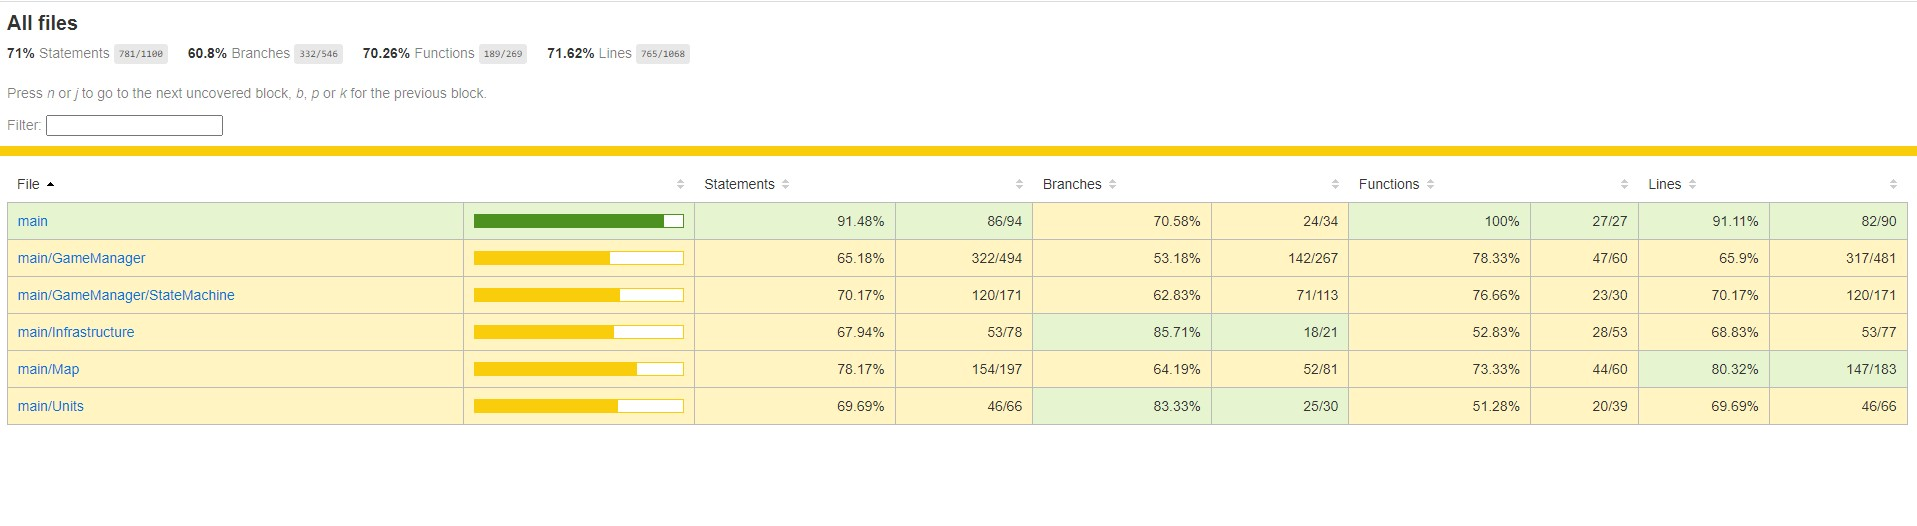
\includegraphics[scale=0.35]{data/couverture_test_1.jpg}
    \caption{Couverture générale du backend}
\end{figure}

On peut voir le pourcentage de couverture de chaque fichier. On peut aussi aller plus dans les détails et regarder ligne par ligne pour être sûr qu'absolument tout le code soit testé.

\begin{figure}[H]
    \centering
    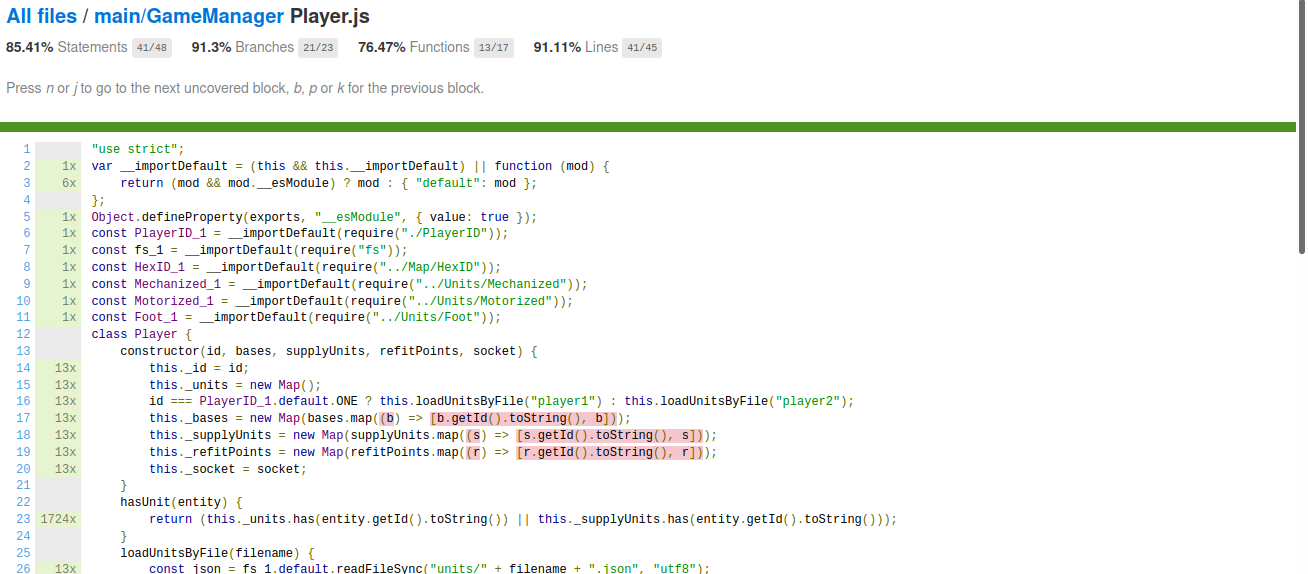
\includegraphics[scale=0.3]{data/couverture_test_2.png}
    \caption{Couverture d'un fichier}
\end{figure}

La couverture du code n'implique pas des tests de qualité. Après quelques recherches nous avons trouvé qu'une couverture minimale de bonne qualité dépasse les 80\%. Nous nous sommes donc fixés d'au moins atteindre ce pourcentage.